% =====================================================================
%  Παρουσίαση — Βελτιστοποίηση Μενού Εστιατορίου (LP & MIP + Δυϊκότητα)
%  Μεταγλώττιση:  lualatex presentation.tex   (x2)
% =====================================================================
\documentclass[aspectratio=169,11pt]{beamer}
\usetheme{Madrid}
\usecolortheme{whale}
\setbeamertemplate{navigation symbols}{}
\setbeamertemplate{caption}[numbered]

\usepackage{amsmath,amssymb}
\usepackage{fontspec}
\usepackage{unicode-math}
\setmathfont{TeX Gyre Termes Math}
\usepackage{polyglossia}
\setmainlanguage{greek}
\setotherlanguage{english}
\setmainfont{GFS Neohellenic}
\setsansfont{GFS Neohellenic}  % το beamer χρησιμοποιεί την οικογένεια sans
% Διόρθωση false-negative ελέγχου σεναρίου της polyglossia για τις γραμματοσειρές GFS.
\ExplSyntaxOn
\cs_set:cpn { polyglossia@addfontfeature@script:nn } #1#2 {
  \tl_if_empty:nF {#2} { \addfontfeature{Script=#2} }
}
\ExplSyntaxOff
\newcommand{\en}[1]{\textenglish{#1}}

\usepackage{booktabs}
\usepackage{graphicx}
\usepackage{xcolor}
\definecolor{navy}{HTML}{1F4E78}
\definecolor{orange}{HTML}{C55A11}
\definecolor{green}{HTML}{2E7D32}
\definecolor{red}{HTML}{B00020}

\setbeamercolor{structure}{fg=navy}
\setbeamercolor{title}{fg=white}
\setbeamerfont{title}{series=\bfseries}
\setbeamertemplate{itemize item}{\color{navy}\textbullet}
\setbeamertemplate{itemize subitem}{\color{orange}--}

\title[Βελτιστοποίηση Μενού]{Βελτιστοποίηση Μενού Εστιατορίου}
\subtitle{Γραμμικός \& Μικτός Ακέραιος Προγραμματισμός --- με Δυϊκή Ανάλυση}
\author[Ε.Χ. Λιαποδημήτρης]{Ευστάθιος Χρυσοβαλάντης Λιαποδημήτρης \\ \small ΑΜ 1100923}
\institute[]{Γραμμική \& Συνδυαστική Βελτιστοποίηση}
\date{Ιούλιος 2026}

\begin{document}

% ---- 1 ---------------------------------------------------------------
\begin{frame}[plain]
  \titlepage
\end{frame}

% ---- 2 ---------------------------------------------------------------
\begin{frame}{Περίγραμμα παρουσίασης}
  \tableofcontents
\end{frame}

% =====================================================================
\section{Το πρόβλημα}
\begin{frame}{Το πρόβλημα: σχεδιασμός ημερήσιου μενού}
  Ο διαχειριστής ενός εστιατορίου καλείται να απαντήσει \emph{ταυτόχρονα} σε τρία
  ερωτήματα:
  \begin{enumerate}
    \item \textbf{Ποια} πιάτα θα προσφέρει σήμερα;
    \item \textbf{Πόσες μερίδες} θα παραχθούν από κάθε πιάτο;
    \item \textbf{Πώς} κατανέμεται ο χρόνος του προσωπικού;
  \end{enumerate}
  \vfill
  \begin{block}{Στόχος}
    Μεγιστοποίηση του ημερήσιου \textbf{μεικτού κέρδους} = έσοδα $-$ μεταβλητό
    κόστος (υλικά, εργασία, σπατάλη) $-$ πάγια κόστη προετοιμασίας.
  \end{block}
  \vfill
  \footnotesize \textbf{Στενός πόρος:} ο \emph{χρόνος εργασίας} της κουζίνας ---
  όλα τα πιάτα ανταγωνίζονται για τις ίδιες $H=65$ ώρες/ημέρα.
\end{frame}

\section{Βιβλιογραφία}
\begin{frame}{Βιβλιογραφικό πλαίσιο}
  \begin{block}{Ιστορικές ρίζες}
    \begin{itemize}
      \item \textbf{\en{Stigler} (1945)} --- το αρχικό \emph{πρόβλημα διατροφής}
        (\en{diet problem})~\cite{stigler}.
      \item \textbf{\en{Dantzig} (1963)} --- Γραμμικός Προγραμματισμός \& μέθοδος
        \en{simplex}~\cite{dantzig}· το \en{diet problem} ήταν από τις πρώτες
        μεγάλες εφαρμογές της.
    \end{itemize}
  \end{block}
  \begin{block}{Θεωρητικά εργαλεία που αξιοποιούμε}
    \begin{itemize}
      \item Δυϊκότητα \& συμπληρωματική χαλαρότητα: \textbf{\en{Bertsimas \&
        Tsitsiklis} (1997)}~\cite{bertsimas}.
      \item Ανάλυση εύρους (\en{ranging}): \textbf{\en{Winston} (2004)}~\cite{winston}.
      \item \en{Branch \& bound} \& ακέραιος προγραμματισμός: \textbf{\en{Land \&
        Doig} (1960)}~\cite{landdoig}, \textbf{\en{Wolsey} (1998)}~\cite{wolsey}.
    \end{itemize}
  \end{block}
\end{frame}

\begin{frame}{Οι τρεις εργασίες αναφοράς --- τι αντλούμε, τι αλλάζουμε}
  \scriptsize
  \begin{tabular}{@{}p{2.6cm}p{4.2cm}p{5.4cm}@{}}
    \toprule
    \textbf{Εργασία} & \textbf{Μεθοδολογία} & \textbf{Στην παρούσα εργασία}\\
    \midrule
    \textbf{\en{Razak et al.}}~\cite{razak} & Συνεχές \en{LP}, ελαχιστοποίηση
      κόστους, διατροφικοί περιορισμοί & \emph{Αντλούμε} το συνεχές \en{LP} πόρων
      (Μοντέλο Α)· \emph{αλλάζουμε} σε μεγιστοποίηση κέρδους / περιορισμό εργασίας\\
    \addlinespace
    \textbf{\en{Sholeha et al.}}~\cite{sholeha} & Δυαδικές $0/1$ επιλογής εδέσματος
      (\en{Boolean ILP}) & \emph{Αντλούμε} το $y_d\in\{0,1\}$· \emph{αλλάζουμε} σε
      \emph{μικτό} με πάγια κόστη \& συνεχή παραγωγή $x_d$\\
    \addlinespace
    \textbf{\en{Silva et al.}}~\cite{silva} & \en{ILP} με περιορισμούς
      ποικιλίας/πλήθους & \emph{Αντλούμε} το $N_{\min}\le\sum y_d\le N_{\max}$·
      \emph{αλλάζουμε} σε \emph{σχεδιαστική} παράμετρο που αποτιμούμε\\
    \bottomrule
  \end{tabular}
  \vfill
  \footnotesize\textbf{Διαφοροποίηση:} οπτική \emph{παραγωγού} (κερδοφορία)· στενός
  πόρος ο \emph{χρόνος}· \emph{σπατάλη} \& \emph{πάγια} κόστη· σχεδιασμός \emph{δύο
  επιπέδων} με πλήρη \textbf{δυϊκή \& παραμετρική ανάλυση}.
\end{frame}

% =====================================================================
\section{Δεδομένα \& κοστολόγηση}
\begin{frame}{Η βάση δεδομένων}
  \begin{columns}[T]
    \begin{column}{0.5\textwidth}
      \begin{block}{Μεγέθη}
        \begin{itemize}
          \item \textbf{52} πρώτες ύλες (τιμές 2026)
          \item \textbf{21} υποψήφια πιάτα ελληνικής κουζίνας
        \end{itemize}
      \end{block}
      \begin{block}{Πηγές τιμών}
        \footnotesize ΟΚΑΑ (χονδρική), Παρατηρητήριο Τιμών / e-Καταναλωτής,
        αλυσίδες Σ/Μ.
      \end{block}
    \end{column}
    \begin{column}{0.5\textwidth}
      \begin{block}{Καθολικές παράμετροι}
        \footnotesize
        \begin{tabular}{@{}lr@{}}
          \toprule
          Παράμετρος & Τιμή \\ \midrule
          Εργατοώρες $H$ & 65,0 ώρες \\
          Ωρομίσθιο $w$ & 7,80 €/ώρα \\
          Σπατάλη $\alpha$ & 6\% \\
          Πλήθος μενού $N_{\min}/N_{\max}$ & 6 / 10 \\
          \bottomrule
        \end{tabular}
      \end{block}
    \end{column}
  \end{columns}
\end{frame}

\begin{frame}{Από τη συνταγή στην κοστολόγηση}
  Για κάθε πιάτο $d$ (τιμή $P_d$, χρόνος $t_d$ λεπτά, συνταγή $\{(i,q_{d,i})\}$):
  \begin{align*}
    \mu_d &= \textstyle\sum_i q_{d,i}\,\pi_i && \text{(υλικά)} &
    \lambda_d &= \tfrac{t_d}{60}w && \text{(εργασία)}\\
    \sigma_d &= \mu_d\,\alpha && \text{(σπατάλη)} &
    C_d &= \mu_d+\lambda_d+\sigma_d && \text{(μεταβλητό)}
  \end{align*}
  \[
    m_d = P_d - C_d \quad\text{(περιθώριο)},\qquad
    \rho_d = \frac{m_d}{t_d/60}\quad\text{(περιθώριο ανά \textbf{εργατοώρα})}
  \]
  \begin{alertblock}{Η παρατήρηση-κλειδί}
    \small
    \begin{tabular}{@{}lrrr@{}}
      & περιθώριο $m$ & χρόνος $t$ & $\rho$ (€/ώρα)\\
      \midrule
      Γαρίδες σαγανάκι & 10,09 € & 12΄ & \textbf{50,46} \\
      Μουσακάς & 4,44 € & 22΄ & \textbf{12,10} \\
    \end{tabular}\\[2pt]
    Ο Μουσακάς \emph{είναι} κερδοφόρος --- απλώς αποδίδει λιγότερο \emph{ανά ώρα}.
  \end{alertblock}
\end{frame}

% =====================================================================
\section{Τα δύο μοντέλα}
\begin{frame}{Μοντέλο Α --- Γραμμικός Προγραμματισμός (\en{LP})}
  \textbf{Μεταβλητές:} $x_d\ge 0$ = μερίδες πιάτου $d$/ημέρα (συνεχείς).
  \begin{block}{}
  \[
    \max\; Z_{\mathrm{LP}} = \sum_{d\in D} m_d\,x_d
  \]
  \vspace{-1.2em}
  \begin{align*}
    \text{υπό:}\quad \sum_{d\in D}\tfrac{t_d}{60}\,x_d &\le H && \text{(εργατοώρες)}\\
    0 \le x_d &\le D_d^{\max} && \forall d \quad\text{(ζήτηση)}
  \end{align*}
  \end{block}
  \begin{itemize}
    \item Μοναδικός συνδετικός περιορισμός: ο \textbf{χρόνος}.
    \item Δεν υπάρχουν πάγια κόστη ούτε όριο πλήθους $\Rightarrow$ \emph{χαλάρωση}
      (\en{relaxation}) $\Rightarrow$ \textbf{άνω φράγμα} κέρδους.
  \end{itemize}
\end{frame}

\begin{frame}{Μοντέλο Β --- Μικτός Ακέραιος Προγραμματισμός (\en{MIP})}
  \textbf{Επιπλέον:} δυαδικές $y_d\in\{0,1\}$ = ένταξη πιάτου στο μενού.
  \begin{block}{}
  \[
    \max\; Z_{\mathrm{MIP}} = \sum_{d\in D} m_d\,x_d - \sum_{d\in D} f_d\,y_d
  \]
  \vspace{-1.2em}
  \begin{align*}
    x_d &\le D_d^{\max} y_d, \quad x_d \ge D_d^{\min} y_d && \forall d
      \quad\text{(σύζευξη, \en{Big-M}$=D_d^{\max}$)}\\
    N_{\min} \le \textstyle\sum_d y_d &\le N_{\max} && \text{(μέγεθος μενού)}
  \end{align*}
  \end{block}
  \begin{itemize}
    \item \emph{Παραγωγή μόνο αν επιλεγεί}· ελάχιστη παρτίδα αν επιλεγεί.
    \item Το πλήθος (6--10) είναι \textbf{σχεδιαστική επιλογή}, όχι φυσικός νόμος.
  \end{itemize}
\end{frame}

\begin{frame}{Πώς συνδέονται τα δύο μοντέλα;}
  Επιλύονται \textbf{ανεξάρτητα}· η σχέση τους είναι εννοιολογική και αναλύει το
  «κόστος πρακτικότητας»:
  \begin{block}{Αποσύνθεση της διαφοράς}
  \[
  \underbrace{1976{,}41}_{\en{LP}\ \text{(άνω φράγμα)}}
  - \underbrace{1709{,}53}_{\en{MIP}\ \text{(υλοποιήσιμο)}}
  = \underbrace{25{,}88}_{\substack{\text{ακεραιότητα}\\\text{\& πληθικότητα}}}
  + \underbrace{241{,}00}_{\text{πάγια κόστη}}
  = 266{,}88\ €
  \]
  \end{block}
  \begin{itemize}
    \item Το μεγαλύτερο μέρος της «θυσίας» (241 €) οφείλεται στα \textbf{πάγια κόστη}.
    \item \small Επιλύτης: \en{PuLP} + \en{COIN-OR CBC}~\cite{coincbc} (\en{simplex} /
      \en{branch \& bound}).
  \end{itemize}
\end{frame}

\begin{frame}{\en{Branch \& bound}: το διάκενο ακεραιότητας}
  Ο \en{branch \& bound}~\cite{landdoig,wolsey} ξεκινά από τη \emph{γραμμική
  χαλάρωση} του \en{MIP} ($y_d\in[0,1]$ αντί $\{0,1\}$) --- το άνω φράγμα στη ρίζα:
  \begin{block}{}
  \[
  \underbrace{Z_{\text{χαλάρ.}} = 1715{,}88}_{\text{ρίζα, } y\in[0,1]}
  \;\;\ge\;\;
  \underbrace{Z_{\mathrm{MIP}} = 1709{,}53}_{\text{ακέραιο}},\qquad
  \text{διάκενο} = 6{,}35\ € \;(0{,}37\%)
  \]
  \end{block}
  \begin{itemize}
    \item Πολύ \textbf{στενό} διάκενο: στη ρίζα, \emph{μόνο δύο} πιάτα είναι
      κλασματικά (Γιουβέτσι $0{,}58$, Κεφτέδες $0{,}42$).
    \item Ο \en{B\&B} διακλαδώνεται σε αυτά για να τα κάνει $0/1$ --- σχεδόν ακαριαία.
    \item \small Προσοχή: το Μοντέλο Α (1976 €) είναι \emph{πιο χαλαρό} φράγμα
      (αγνοεί \& πάγια κόστη \& πληθικότητα).
  \end{itemize}
\end{frame}

% =====================================================================
\section{Αποτελέσματα}
\begin{frame}{Κατάταξη αποδοτικότητας ανά εργατοώρα}
  \centering
  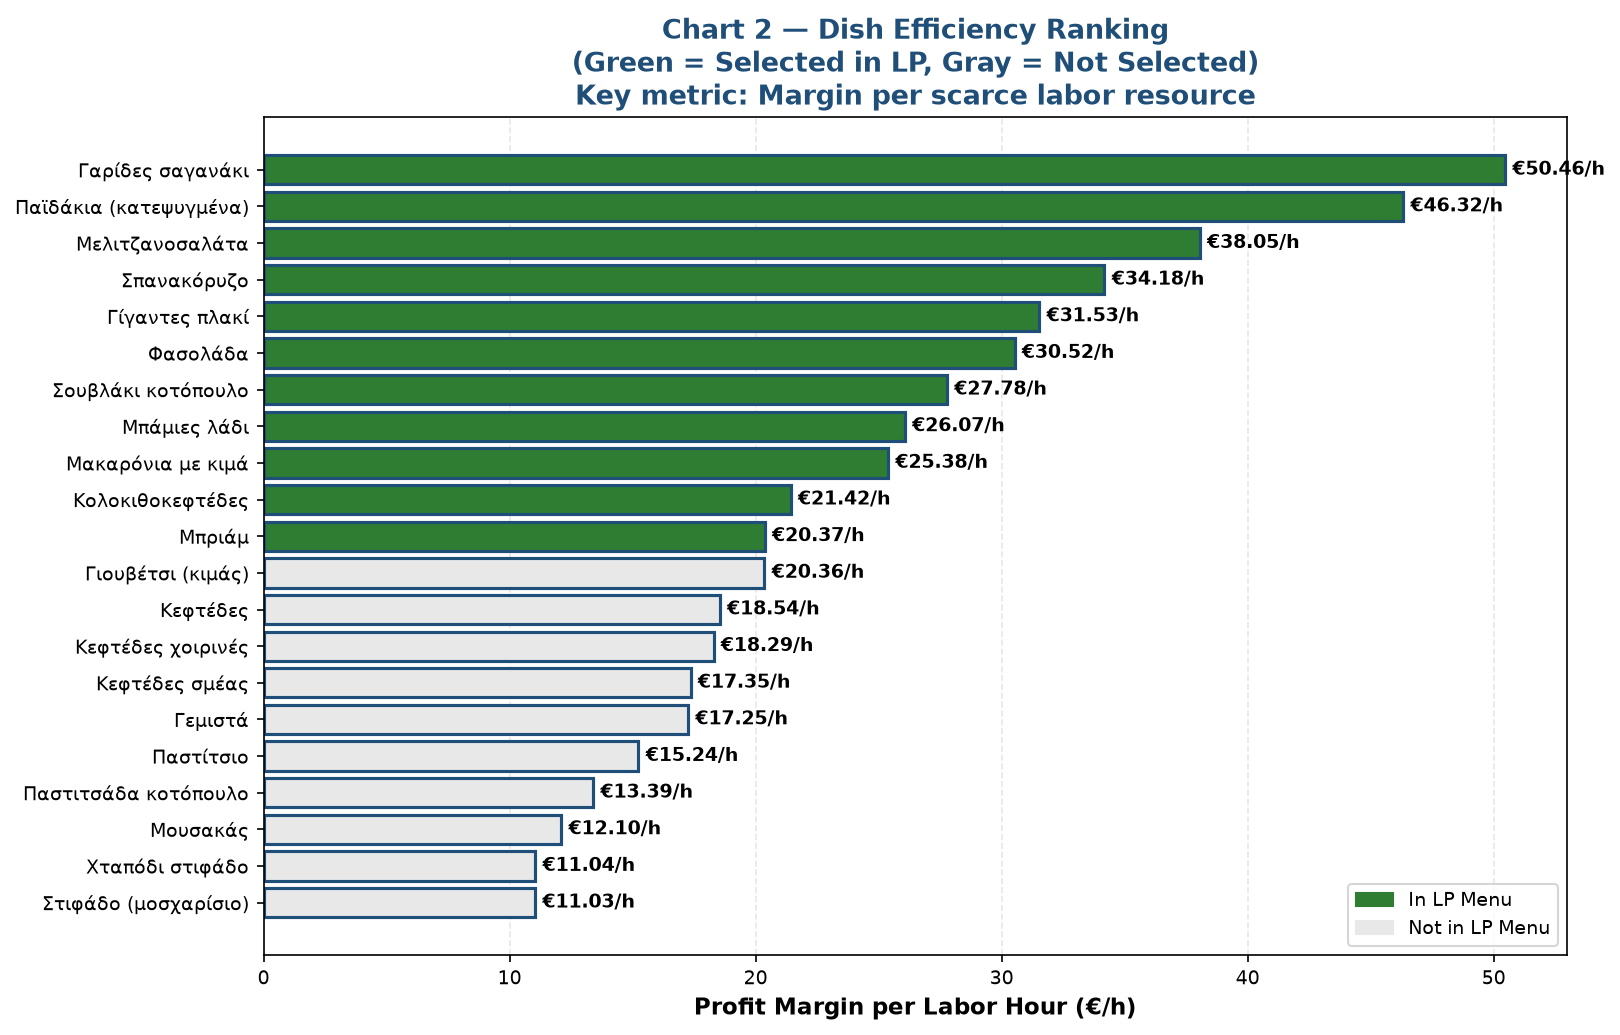
\includegraphics[height=0.8\textheight]{chart_02_efficiency_ranking.png}
\end{frame}

\begin{frame}{Το βέλτιστο μενού του \en{MIP}}
  \begin{columns}[c]
    \begin{column}{0.62\textwidth}
      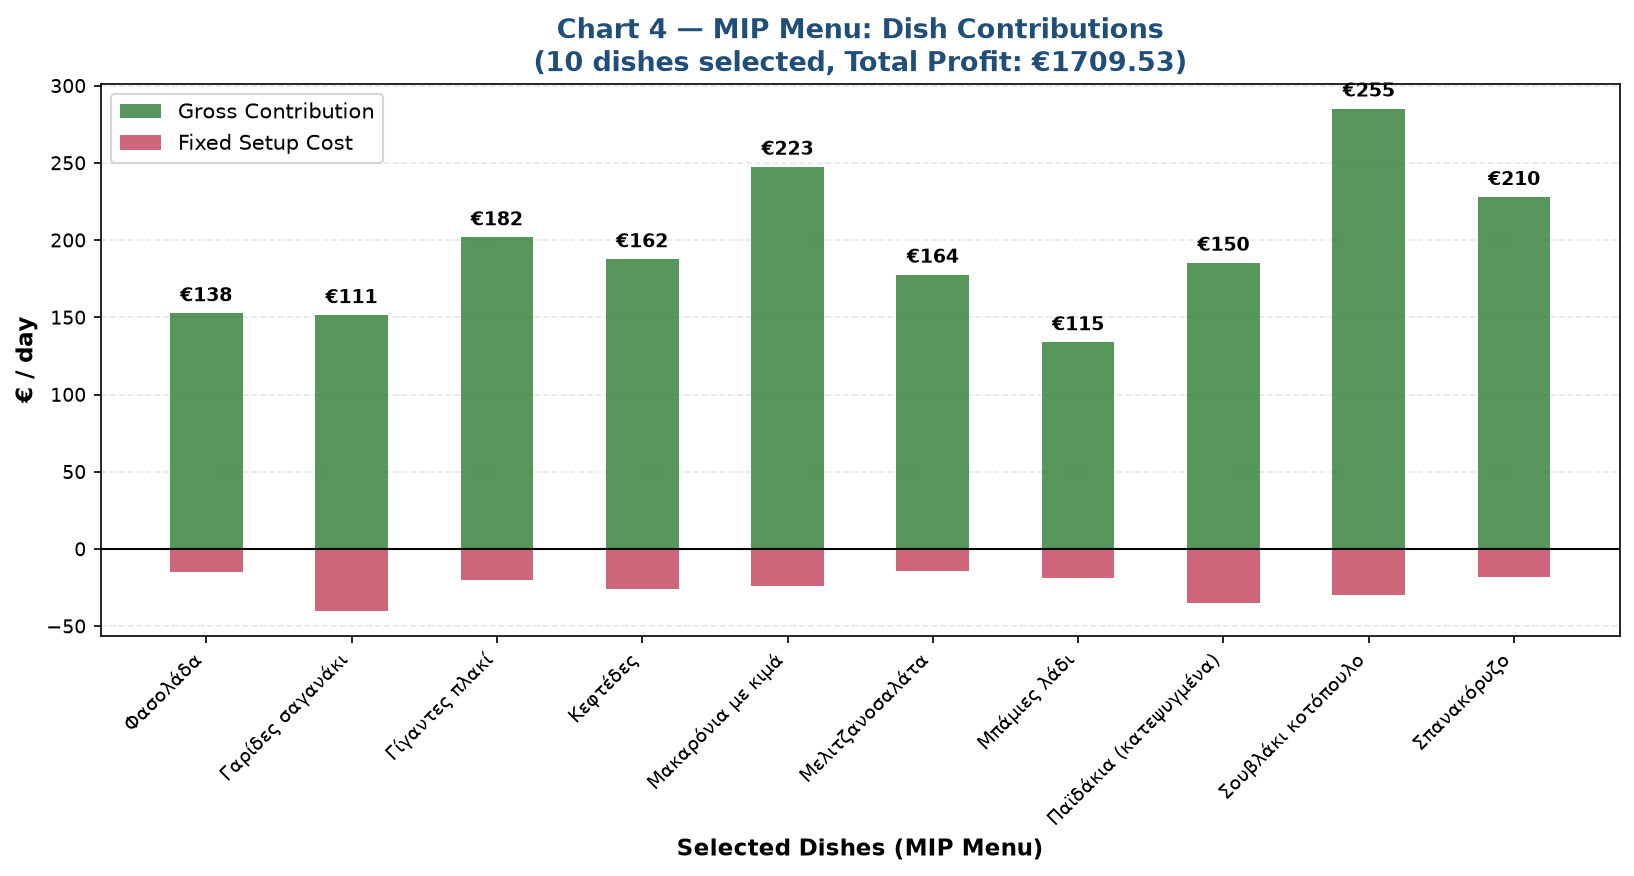
\includegraphics[width=\textwidth]{chart_04_mip_contributions.png}
    \end{column}
    \begin{column}{0.38\textwidth}
      \small
      \begin{itemize}
        \item \textbf{10 πιάτα} (το όριο $N_{\max}$).
        \item Κέρδος \textbf{1709,53 €}/ημέρα.
        \item Όλα με \emph{θετική} καθαρή συνεισφορά.
        \item Η παραγωγή «κολλάει» στο όριο ζήτησης $D_d^{\max}$ για τα αποδοτικά πιάτα.
      \end{itemize}
    \end{column}
  \end{columns}
\end{frame}

% =====================================================================
\section{Δυϊκότητα}
\begin{frame}{Δυϊκότητα: το δυϊκό πρόβλημα}
  Σε κάθε περιορισμό αντιστοιχεί μια \emph{σκιώδης τιμή}: εργασία $u\ge0$, ζήτηση
  $v_d\ge0$.
  \begin{block}{Δυϊκό \en{LP}}
  \vspace{-0.6em}
  \begin{align*}
    \min\; W &= H\,u + \sum_{d\in D} D_d^{\max}\, v_d\\
    \text{υπό:}\quad \tfrac{t_d}{60}\,u + v_d &\ge m_d \qquad \forall d\in D
  \end{align*}
  \end{block}
  \begin{itemize}
    \item Αριστερό μέλος = \textbf{αποτιμημένο κόστος ευκαιρίας} μιας μερίδας του $d$.
    \item Πρέπει να καλύπτει τουλάχιστον το περιθώριο $m_d$.
  \end{itemize}
\end{frame}

\begin{frame}{Ισχυρή δυϊκότητα \& σκιώδης τιμή εργασίας}
  \begin{block}{Ισχυρή δυϊκότητα (αριθμητική επιβεβαίωση)}
    \[
      Z^\star_{\mathrm{LP}} = W^\star = 1976{,}41\ €,\qquad |Z^\star - W^\star| < 10^{-3}.
    \]
  \end{block}
  \begin{alertblock}{Σκιώδης τιμή της εργασίας}
    \[
      u^\star = 20{,}37\ €/\text{ώρα} \;\gg\; w = 7{,}80\ €/\text{ώρα}
    \]
    Κάθε επιπλέον εργατοώρα αποδίδει \textbf{$+12{,}6$ €} καθαρού περιθωρίου
    $\Rightarrow$ η πρόσληψη προσωπικού είναι σαφώς \emph{κερδοφόρα}.
  \end{alertblock}
  \footnotesize Επιπλέον, ικανοποιούνται πλήρως οι συνθήκες
  \emph{συμπληρωματικής χαλαρότητας} (η εργασία εξαντλείται· $v_d^\star>0$ μόνο στο
  όριο ζήτησης· $r_d\ne0$ μόνο για μη παραγόμενα).
\end{frame}

\begin{frame}{Μειωμένο κόστος: γιατί αποκλείεται ο Μουσακάς}
  \begin{columns}[c]
    \begin{column}{0.6\textwidth}
      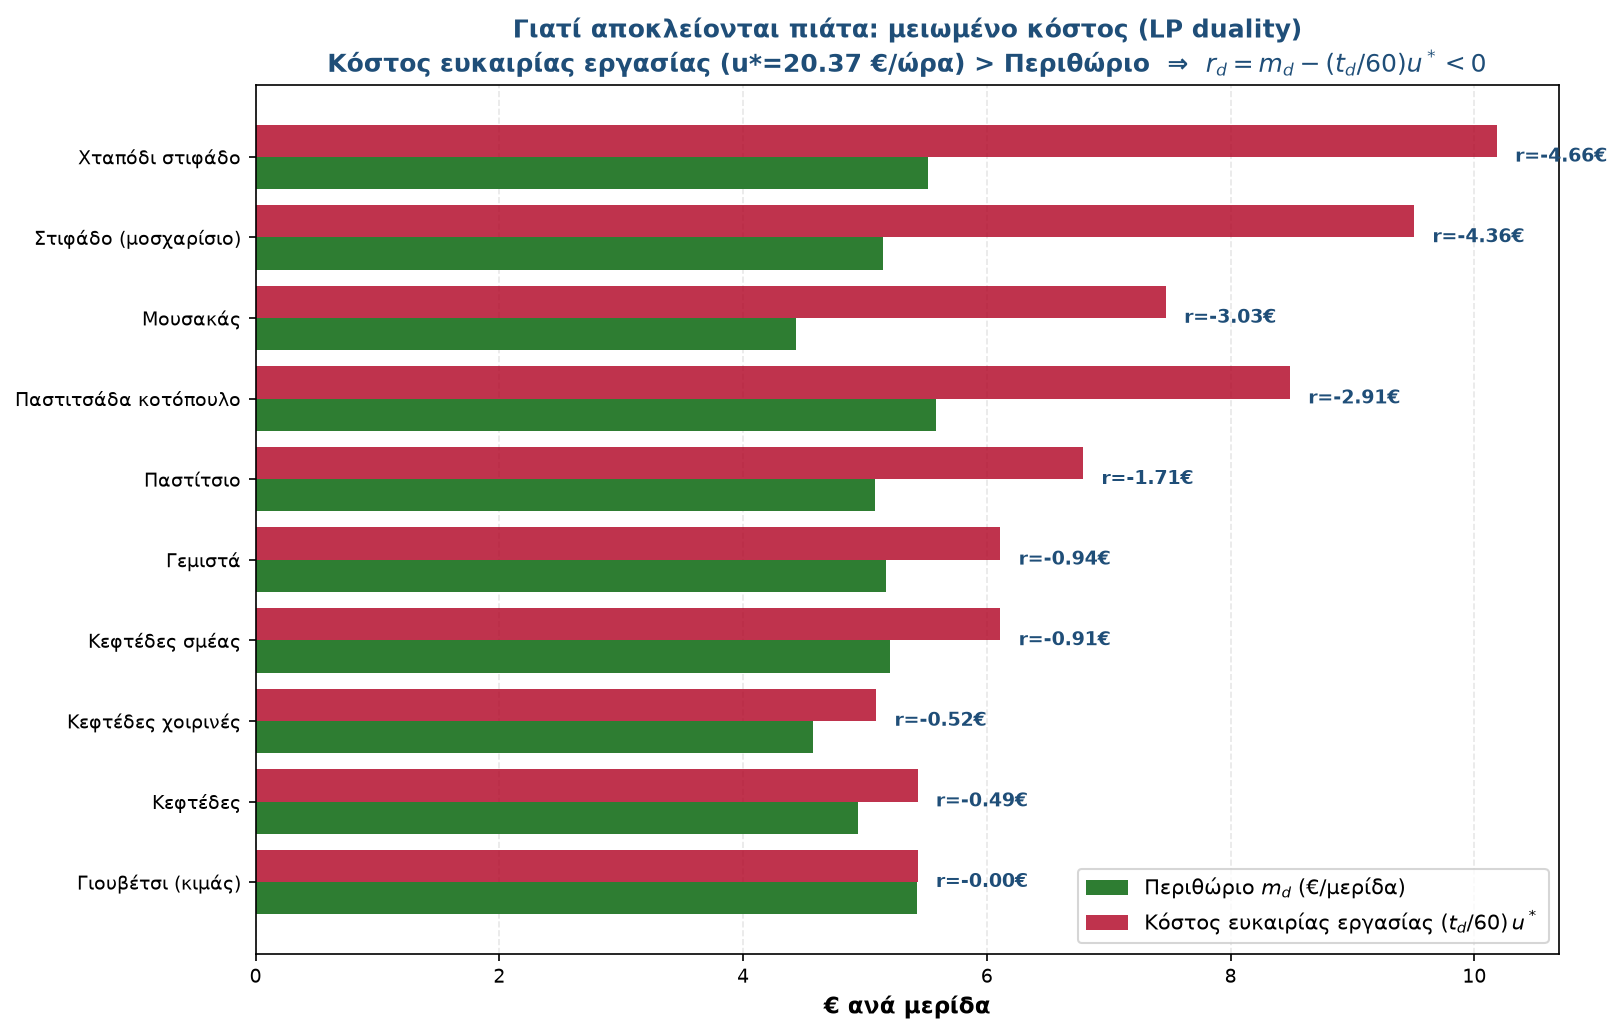
\includegraphics[width=\textwidth]{chart_09_reduced_cost.png}
    \end{column}
    \begin{column}{0.4\textwidth}
      \small
      \[ r_d = m_d - \tfrac{t_d}{60}u^\star \le 0 \]
      Για τον Μουσακά:
      \[ r = 4{,}44 - \tfrac{22}{60}(20{,}37) = -3{,}03\ € \]
      \begin{itemize}
        \item Το $|r_d|$ = \textbf{κόστος ευκαιρίας}.
        \item Το κόστος ευκαιρίας του χρόνου ($7{,}47$ €) \emph{ξεπερνά} το περιθώριο.
        \item Δεν χάνει χρήματα --- απλώς ο χρόνος αξίζει περισσότερα αλλού.
      \end{itemize}
    \end{column}
  \end{columns}
\end{frame}

\section{Παραμετρική ανάλυση}
\begin{frame}{Εύρος δεξιού μέλους: πόσο ισχύει η σκιώδης τιμή;}
  \begin{columns}[c]
    \begin{column}{0.62\textwidth}
      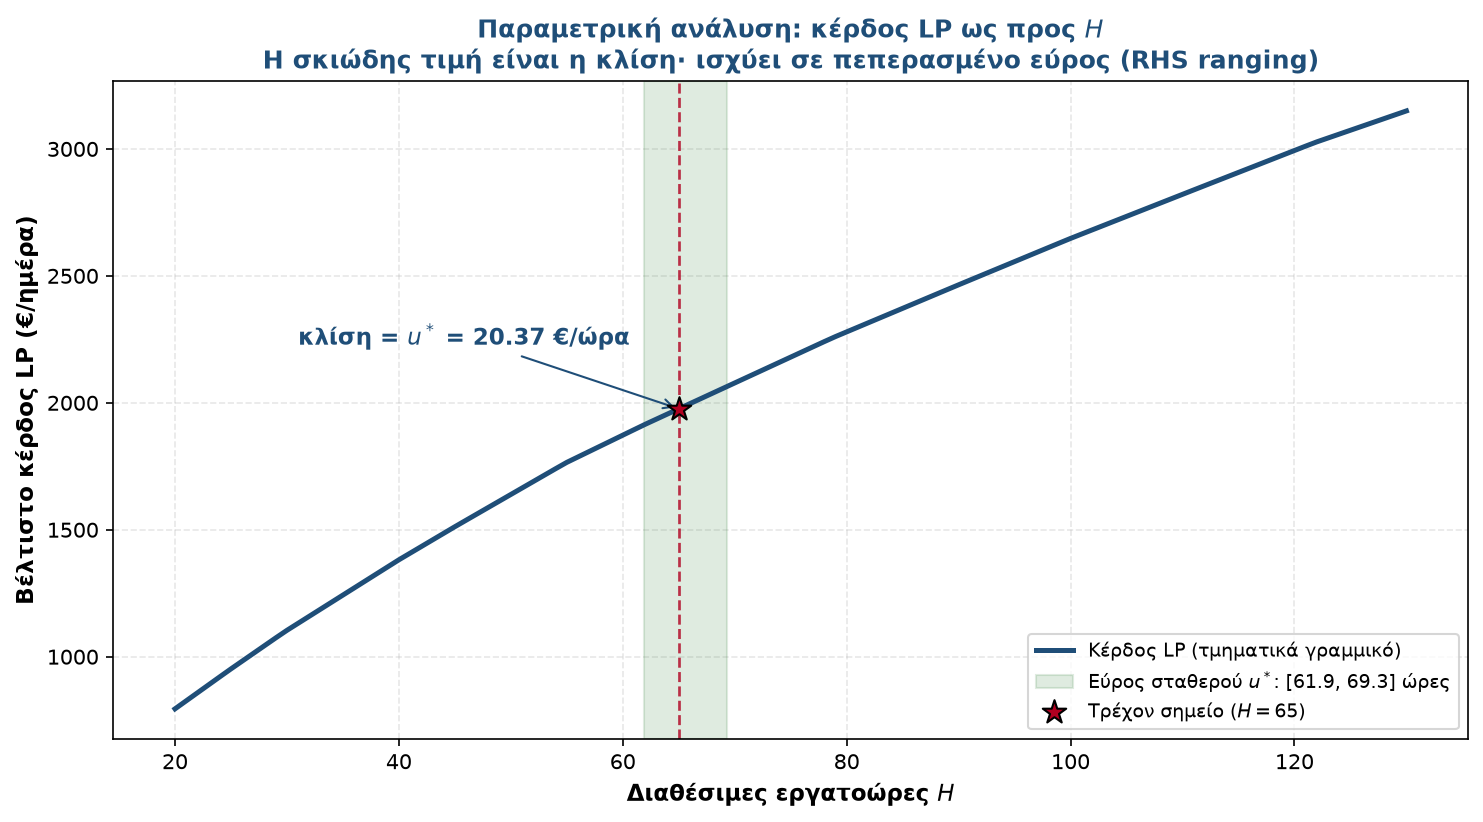
\includegraphics[width=\textwidth]{chart_11_parametric_labor.png}
    \end{column}
    \begin{column}{0.38\textwidth}
      \small
      Το κέρδος(H) είναι \emph{τμηματικά γραμμικό}· η κλίση κάθε τμήματος είναι η
      σκιώδης τιμή.
      \begin{block}{Εύρος ισχύος του $u^\star$}
        \[ H \in [\,61{,}88,\ 69{,}35\,]\ \text{ώρες} \]
        (μείωση $3{,}12$, αύξηση $4{,}35$ ώρες)
      \end{block}
      Πέρα από αυτό, η βάση αλλάζει και το $u^\star$ \emph{μειώνεται} (η καμπύλη
      λυγίζει).
    \end{column}
  \end{columns}
\end{frame}

\begin{frame}{Εύρος συντελεστών: πόσο αντέχει κάθε περιθώριο;}
  \small
  Πόσο μπορεί να αλλάξει το περιθώριο $m_d$ χωρίς να αλλάξει η βέλτιστη λύση $x^\star$;
  \begin{columns}[T]
    \begin{column}{0.5\textwidth}
      \begin{block}{Παραγόμενα πιάτα}
        Αύξηση: $\infty$ (μένουν στο μενού).\\
        Μείωση: πεπερασμένη --- π.χ. οι Γαρίδες αντέχουν πτώση \textbf{6,02 €}.
      \end{block}
    \end{column}
    \begin{column}{0.5\textwidth}
      \begin{alertblock}{Αποκλειόμενα πιάτα}
        Επιτρεπτή αύξηση $=|r_d|$ ακριβώς!\\
        Μουσακάς: χρειάζεται \textbf{+3,03 €} περιθώριο για να μπει --- όσο και το
        μειωμένο κόστος του.
      \end{alertblock}
    \end{column}
  \end{columns}
  \vfill
  \centering
  \emph{Η ταύτιση «επιτρεπτή αύξηση $=$ μειωμένο κόστος» επιβεβαιώνει τη συνέπεια
  δυϊκότητας -- ranging.}
\end{frame}

% =====================================================================
\section{Ευαισθησία \& συμπεράσματα}
\begin{frame}{Ανάλυση ευαισθησίας: διαθέσιμες εργατοώρες}
  \begin{columns}[c]
    \begin{column}{0.62\textwidth}
      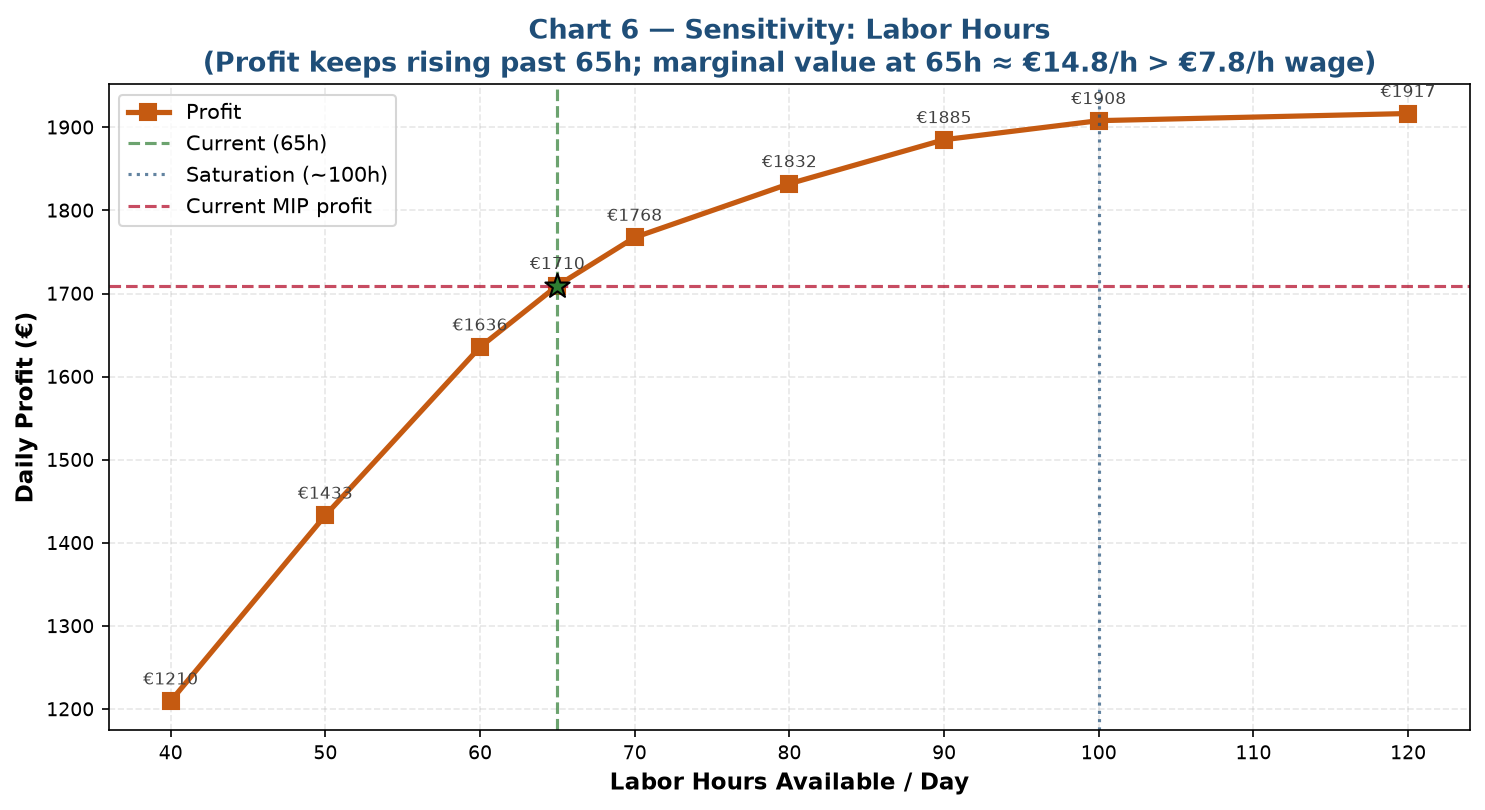
\includegraphics[width=\textwidth]{chart_06_sensitivity_labor.png}
    \end{column}
    \begin{column}{0.38\textwidth}
      \small
      \begin{itemize}
        \item Οριακό όφελος στις 65 ώρες: $\approx 14{,}8$ €/ώρα.
        \item Το κέρδος αυξάνεται \emph{αρκετά πέρα} από τις 65 ώρες.
        \item Κορεσμός γύρω στις $\sim100$ ώρες.
        \item Συνεπές με τη σκιώδη τιμή $u^\star$.
      \end{itemize}
    \end{column}
  \end{columns}
  \vfill
  \footnotesize Επίσης: το \emph{κόστος υλικών} έχει τη μεγαλύτερη επίδραση·
  μείωση σπατάλης 6\%$\to$3\% $\approx +22{,}6$ €/ημέρα ($\sim$8000 €/έτος).
\end{frame}

\begin{frame}{Συζήτηση: τα παραδοσιακά πιάτα δεν είναι ασύμφορα}
  \begin{itemize}
    \item Ο αποκλεισμός του Μουσακά είναι θέμα \textbf{κόστους ευκαιρίας}, όχι ζημίας.
    \item \textbf{Πείραμα:} με άφθονη εργασία ($H=120$):
      \begin{itemize}
        \item με $N_{\max}=10$, ο \textbf{Μουσακάς επανέρχεται} στο μενού·
        \item χωρίς όριο, επιλέγονται 16 πιάτα (\textbf{μαζί με το Γιουβέτσι}),
          κέρδος \textbf{2596,77 €}.
      \end{itemize}
    \item Το ίδιο το μοντέλο τα επανεντάσσει όταν αυξάνεται ο χρόνος.
  \end{itemize}
  \vfill
  \begin{block}{Πρακτική σύσταση}
    Στο τρέχον επίπεδο: προτεραιότητα στα αποδοτικά ανά ώρα πιάτα. Παράλληλα:
    εξέταση αύξησης προσωπικού --- τη δικαιολογεί η σκιώδης τιμή $u^\star=20{,}37$ €/ώρα.
  \end{block}
\end{frame}

\begin{frame}{Συμπεράσματα}
  \begin{enumerate}
    \item Σύστημα \textbf{δύο μοντέλων}: \en{LP} (άνω φράγμα 1976,41 €) και \en{MIP}
      (υλοποιήσιμο 1709,53 €, 10 πιάτα)· διαφορά = 241 € πάγια + 26 € ακεραιότητα.
    \item Ο στενός πόρος είναι ο \textbf{χρόνος}· κρίσιμο μέτρο το $\rho_d$
      (περιθώριο ανά εργατοώρα).
    \item \textbf{Δυϊκότητα:} ισχυρή δυϊκότητα επιβεβαιωμένη· σκιώδης τιμή εργασίας
      $u^\star=20{,}37$ €/ώρα· μειωμένα κόστη εξηγούν \emph{ποσοτικά} κάθε αποκλεισμό.
    \item \textbf{Παραμετρική ανάλυση:} το $u^\star$ ισχύει σε $[61{,}9, 69{,}4]$ ώρες·
      διάκενο ακεραιότητας μόλις $0{,}37\%$ (\en{branch \& bound}).
    \item Η ανάλυση ευαισθησίας \& τα πειράματα $H=120$ επιβεβαιώνουν όλα τα παραπάνω.
  \end{enumerate}
  \vfill
  \centering
  \structure{\Large Ευχαριστώ! \normalsize\\[4pt] Ερωτήσεις;}
\end{frame}

% ---------------------------------------------------------------------
\appendix
\begin{frame}[allowframebreaks]{Αναφορές}
  \footnotesize
  \begin{thebibliography}{9}
    \bibitem{stigler} \en{Stigler, G.\,J. (1945). The Cost of Subsistence.
      \textit{J.\ Farm Economics} 27(2), 303--314.}
    \bibitem{dantzig} \en{Dantzig, G.\,B. (1963). \textit{Linear Programming and
      Extensions.} Princeton Univ.\ Press.}
    \bibitem{bertsimas} \en{Bertsimas, D.\ \& Tsitsiklis, J.\,N. (1997).
      \textit{Introduction to Linear Optimization.} Athena Scientific.}
    \bibitem{winston} \en{Winston, W.\,L. (2004). \textit{Operations Research}
      (4th ed.). Brooks/Cole.}
    \bibitem{landdoig} \en{Land, A.\,H.\ \& Doig, A.\,G. (1960). An Automatic Method
      of Solving Discrete Programming Problems. \textit{Econometrica} 28(3), 497--520.}
    \bibitem{wolsey} \en{Wolsey, L.\,A. (1998). \textit{Integer Programming.} Wiley.}
    \bibitem{silva} \en{Silva, A.\ et al. University restaurants menu planning using
      mathematical modelling (ILP).}
    \bibitem{razak} \en{Razak, N.\,A.\ et al. Application of Linear Programming on
      Diet Problem for Kenny Roger's Roaster.}
    \bibitem{sholeha} \en{Sholeha, M.\ et al. Diet-Menu Problem Modelling Based on
      Linear Boolean Approach.}
    \bibitem{coincbc} \en{Forrest, J.\ et al. COIN-OR CBC· Mitchell, S.\ et al.
      PuLP (Python).}
  \end{thebibliography}
\end{frame}

\end{document}
